\section{Příklad 4}
% Jako parametr zadejte skupinu (A-H)
\ctvrtyZadani{C}
\
\textbf{Naznačíme proudy $I_a$, $I_b$, $I_c$, jelikož počítáme metodou smyčkových proudů.}

\begin{figure}[!ht]
    \centering
    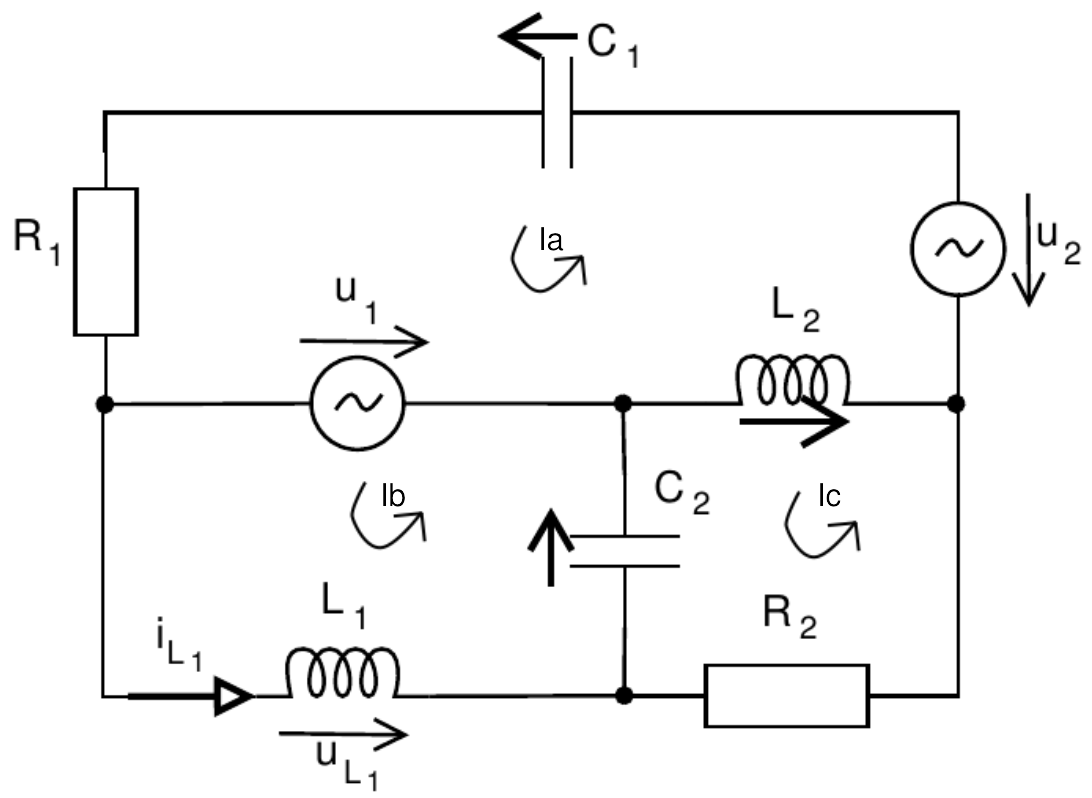
\includegraphics[width=0.9\textwidth, keepaspectratio]
    {/home/tjoslef/skola/zapisky/vut/IEL/projekt/sablona_reseni/fig/priklad4.png}
    \caption{Schéma obvodu s naznačenými smyčkovými proudy.}
\end{figure}

\textbf{Sestavíme si rovnici podle smyček:}

\[
    I_a: \quad Z_{c1} + R_1 \cdot I_a + Z_{l2} \cdot (I_c - I_b) + U_1 - U_2 = 0
\]

\[
    I_b: \quad -U_1 + I_b \cdot Z_{l1} + Z_{l2} \cdot (I_b - I_c) = 0
\]

\[
    I_c: \quad -Z_{l2} \cdot (I_a - I_c) - Z_{c2} \cdot (I_b - I_c) + I_c \cdot R_2 = 0
\]

\textbf{Vyjadřime neznáme ktere víme}

\[
    \omega = 2 \cdot \pi \cdot f \quad \Rightarrow \quad \omega = 471.23889803846896
\]

\[
    t = \frac{\pi}{2 \cdot \omega} \quad \Rightarrow \quad t = \frac{1}{333}
\]

\[
    Z_{c1} = \frac{-1j}{\omega \cdot C_1} \quad \Rightarrow \quad Z_{c1} = -9.23j
\]

\[
    Z_{c2} = \frac{-1j}{\omega \cdot C_2} \quad \Rightarrow \quad Z_{c2} = -24.97j
\]

\[
    Z_{l1} = 1j \cdot \omega \cdot L_1 \quad \Rightarrow \quad Z_{l1} =103.67j
\]

\[
    Z_{l2} = 1j \cdot \omega \cdot L_2 \quad \Rightarrow \quad Z_{l2} = 32.99j
\]
\textbf{Ze soustavy rovnic zjistime}
\[
    I_a = 0.0039 - 0.0267j
\]
\[
    I_b = 0.0017 - 0.0413j
\]
\[
    I_c = -0.0053 + 0.0099j
\]
\[
    U_{L1} = I_b \cdot Z_{l1} \quad \Rightarrow \quad U_{L1} = 4.2803
\]
\textbf{Z komplexní části \( U_{L1} \) jsme schopni zjistit fázový posun}
\[
    \Phi = \arctan\left(\frac{\text{imaginarni cast}}{\text{realna cast}}\right) \quad \Rightarrow \quad \Phi = 0.0408
\]

